\chapter{基于自注意力机制的端侧运动想象脑电解码模型设计与验证}
\label{cha:algorithm}

本章围绕受限采集与边缘侧推理条件下的运动想象脑电解码模型设计与验证展开。针对少导联输入适配、模型规模控制和端侧部署需求并存的约束，本文以运动想象脑电的中央区节律特征为生理依据，构建兼顾标准任务准确率、模型规模控制和少导联输入适配的自注意力解码模型，并围绕 22 导参考输入、C3/C4 双导目标输入以及准确率、模型规模和推理耗时等验证口径，对 EdgeMIFormer 的局部窗口自注意力结构、训练配置、剪枝量化部署和导联受限实验结果进行分析。

\section{算法设计目标与端侧约束}
本节从运动想象脑电的信号特征和端侧约束出发，明确中央区导联与左右手任务选择的依据，并统一导联配置、准确率、模型规模、推理耗时以及剪枝量化部署的验证口径，为后续模型设计和实验分析提供边界。

\subsection{运动想象脑电信号特征}
运动想象（Motor Imagery, MI）是指个体在不产生实际肢体运动输出的前提下，在脑内主动表征动作过程的心理活动。对本章算法设计而言，运动想象脑电的关键不在于其完整神经机制，而在于它提供了相对明确的解码对象：感觉运动皮层附近的节律变化、左右手任务中的侧化差异，以及跨被试不完全一致的时空响应模式。本文选择运动想象任务作为模型验证对象，正是因为该任务既具有稳定的中央区生理基础，又能直接对应端侧脑机接口中的主动控制需求。

从空间分布看，左右手运动想象的判别信息主要集中在中央感觉运动区附近，C3 与 C4 通常对应左右手区的侧化响应，Cz 则可能补充中线附近的运动相关信息 \cite{Pfu06,Mcf04}。这一特点决定了本章不能只在标准 22 导设置下讨论模型准确率，还需要进一步观察模型在中央区少导联和 C3/C4 双导条件下的表现。换言之，22 导输入用于提供较完整的参考观测，C3/C4 双导输入则对应端侧硬件目标形态，中间的 8 导和 3 导设置用于连接二者之间的导联压缩过程。

从时间和频率特征看，运动想象脑电主要表现为 $\mu$ 节律和 $\beta$ 节律范围内的事件相关去同步化或同步化变化。此类判别线索通常并非均匀分布在整个试次中，而是集中在有限的时间片段和特定节律范围内。因此，模型需要具备局部时序模式提取能力，同时又不能完全忽略相邻时间片段之间的上下文关系。本章采用卷积前端与局部窗口自注意力结合的结构，正是为了在节律局部性和时间上下文建模之间取得平衡。

\begin{figure}[H]
    \centering
    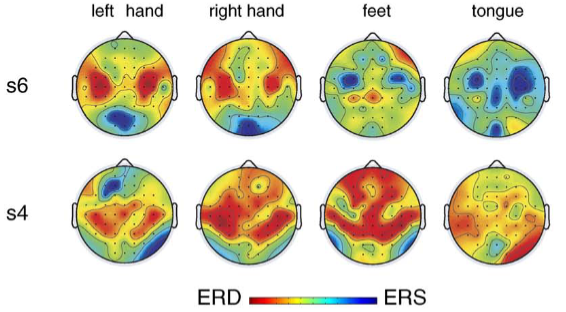
\includegraphics[width=0.68\textwidth]{figures/C1-7_ERD_ERS_topomap.png}
    \caption{不同运动想象类别下 ERD/ERS 现象的头皮地形分布示意\cite{Pfu06}}
    \label{fig:chap4_mi_erd_ers_topomap}
\end{figure}

如图 \ref{fig:chap4_mi_erd_ers_topomap} 所示，不同运动想象类别通常会在感觉运动相关区域诱发差异化的节律抑制与反弹模式，这也为本章围绕运动想象任务开展算法设计提供了明确的生理基础。

除了群体层面的共性之外，运动想象脑电还存在明显个体差异。不同受试者的侧化强度、频带响应和有效时间窗并不完全一致 \cite{Zap20b}。因此，本章模型设计不采用固定的手工通道权重或刚性对称先验，而是通过可学习的时空特征嵌入、自注意力编码和训练增强策略保留个体适配空间。实验报告中同时给出平均最佳准确率和平均历程准确率，也是为了区分单次较优性能与训练过程稳定性。

上述信号特性也决定了本章端侧算法设计需要同时考虑准确率和采集形态。本文面向导联数量、佩戴成本和边缘算力均受限制的端侧系统。标准公开数据集通常采用 22 导或更多导联记录脑电信号，能够提供较完整的空间观测；双导或少导联采集形态则会显著压缩空间信息，改变可稳定支持的任务边界。由此，本章从标准 22 导参考设置出发，进一步分析模型在中央区少导联和 C3/C4 双导条件下的性能变化，为端侧系统选择合适的任务目标和模型配置。

\subsection{多导联输入兼容与验证口径}
本章验证指标由准确率、模型规模、推理开销和导联配置共同构成。标准 22 导四分类设置用于检验模型在较完整空间观测条件下的离线识别表现；C3/C4 双导左右手二分类设置对应更极简的端侧采集形态，用于观察模型在有限空间观测下是否仍能保持具有判别意义的解码性能。两类输入之间的 8 导和 3 导配置主要用于观察导联数量减少时四分类任务准确率的变化趋势，为后续任务类别粒度调整提供经验依据。

分类准确率采用平均最佳准确率（Avg Best Acc）和平均历程准确率（Avg Aver Acc）共同报告。前者反映训练过程中可达到的较优测试性能，后者反映训练历程中的整体稳定水平。模型规模和推理开销通过模型文件大小、近似 MACs/FLOPs 和单样本推理耗时衡量。其中，模型大小影响端侧存储成本，计算量和推理耗时直接影响反馈延迟。本章的部署相关结论限定在模型转换、剪枝量化和推理性能测试证据范围内，不延伸到采集、通信与在线反馈链路的整体验证。

具体实验围绕标准输入参考、模型规模控制和低导联任务收束三条证据链展开。22 导四分类结果用于验证 EdgeMIFormer 在标准运动想象任务中的准确率和模型开销；窗口长度消融、剪枝量化和 RK NPU 推理测试用于分析模型在端侧算力约束下的适配能力；导联逐级约简、C3/C4 双导二分类和 BCI IV 2b 外部验证结果用于判断少导联条件下任务类别粒度的合理选择。

\begin{table}[htbp]
    \centering
    \small
    \caption{端侧运动想象解码的设计约束与验证安排}
    \label{tab:chap4_goal_evidence}
    \begin{tabularx}{\textwidth}{p{2.1cm}p{3.1cm}p{3.5cm}>{\raggedright\arraybackslash}X}
        \hline
        验证维度 & 约束来源 & 模型设计响应 & 对应实验 \\
        \hline
        标准输入准确率 & 22 导四分类提供较完整空间观测，是模型解码能力的参考条件 & 卷积前端提取局部节律特征，局部窗口自注意力建模相邻片段依赖 & 22 导四分类标准结果，EEGNet/EEGConformer 对照 \\
        模型规模与推理耗时 & 端侧设备存储、计算资源和反馈延迟均受限制 & 控制嵌入维度，采用局部窗口自注意力，并结合剪枝与量化完成 RKNN 部署 & 模型大小、FLOPs、RK NPU 推理耗时与量化后准确率 \\
        导联配置与任务类别粒度 & C3/C4 双导压缩空间观测，四分类任务目标可能需要调整 & 保持主干对不同导联数量输入的兼容，并将双导目标任务收束为左右手二分类 & 22/8/3/2 导四分类过渡分析，C3/C4 四分类与二分类对比，BCI IV 2b 外部验证 \\
        \hline
    \end{tabularx}
\end{table}

\section{基于局部窗口自注意力的 EdgeMIFormer 设计}
\subsection{总体结构与设计思路}
EdgeMIFormer 采用卷积前端与局部窗口自注意力相结合的建模路线。给定预处理后的脑电输入，模型首先通过时间卷积和空间卷积提取局部时空表征，再将特征映射为自注意力编码器可处理的序列：
\begin{align}
    \mathbf{X} &\in \mathbb{R}^{C \times T},
    \label{eq:input_signal}
    \\
    \mathbf{Z} &\in \mathbb{R}^{N \times D},
    \label{eq:feature_sequence}
\end{align}
其中，$C$ 表示导联数，$T$ 表示时间采样点数，$N$ 表示序列长度，$D$ 表示特征维度。该结构能够在不同导联配置下保持相同的基本处理流程，因此适合用于比较标准 22 导、中央区少导联和 C3/C4 双导输入。

\begin{figure}[H]
    \centering
    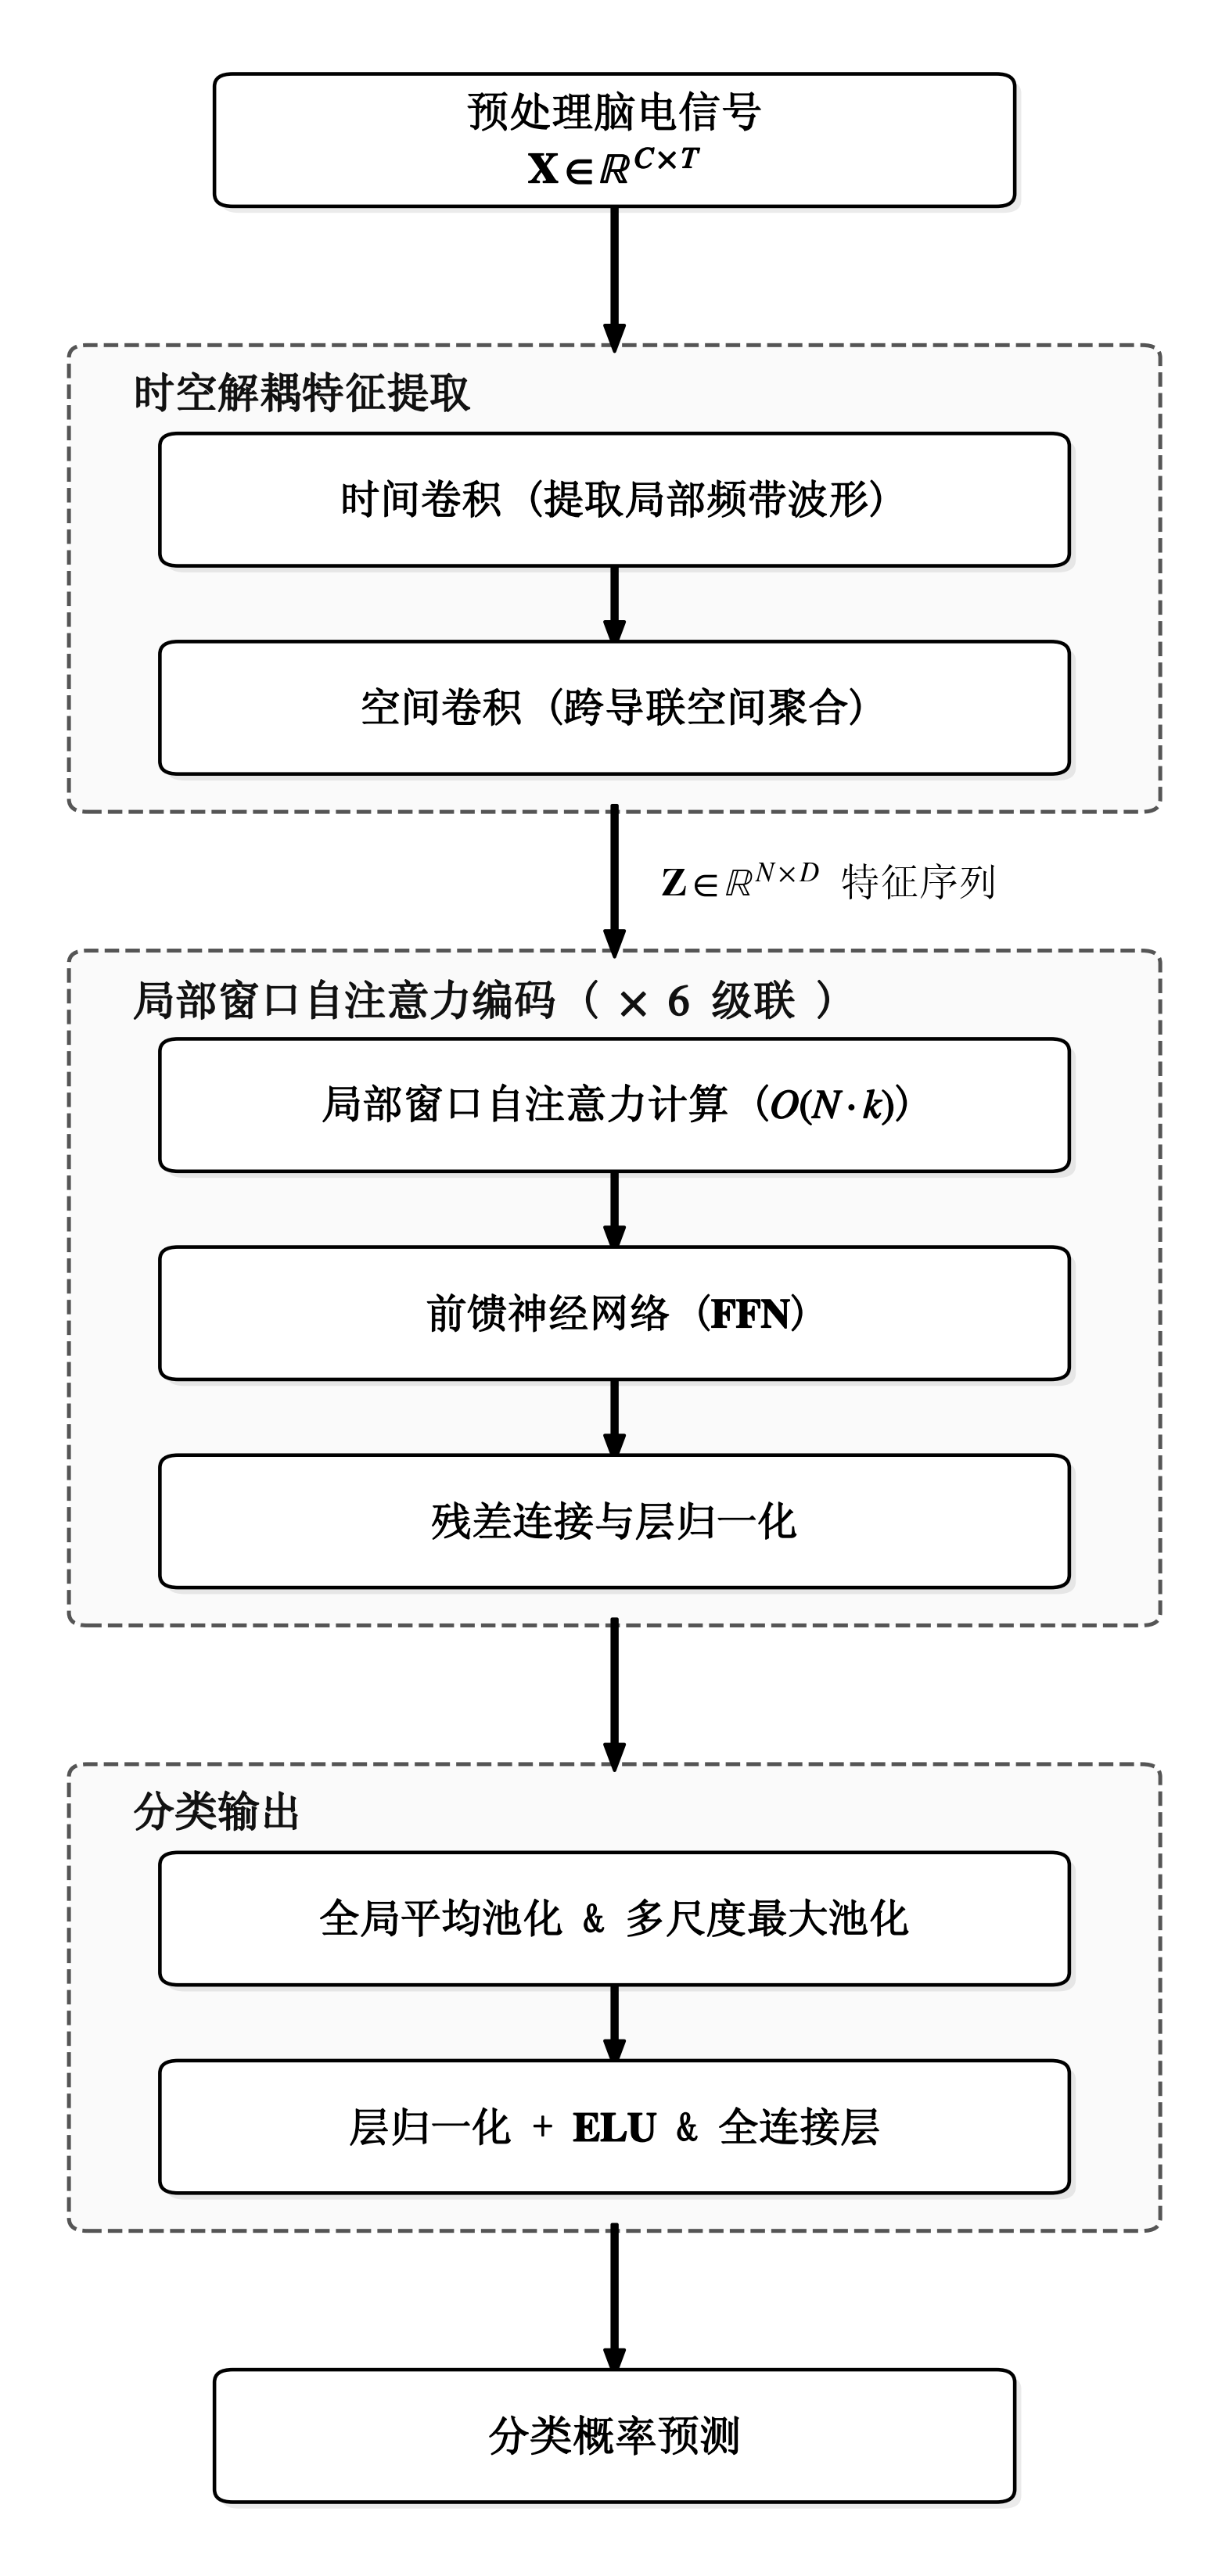
\includegraphics[height=0.56\textheight,keepaspectratio]{EdgeMIFormer_Arch_Rendered.png}
    \caption{EdgeMIFormer 模型架构示意}
    \label{fig:edgemiformer_arch}
\end{figure}

模型设计的核心取向是在分类准确率与模型开销之间建立平衡。卷积前端用于提取运动想象脑电中较稳定的局部时序模式和跨导联关系；局部窗口自注意力用于在较低计算开销下建模相邻特征片段之间的依赖；分类头则根据四分类或二分类任务进行相应调整。该设计使自注意力机制服务于端侧运动想象解码，并为后续少导联输入和任务收束实验提供统一主干。

\begin{table}[htbp]
    \centering
    \small
    \caption{EdgeMIFormer 的主要结构与训练配置}
    \label{tab:edgemiformer_config}
    \begin{tabularx}{\textwidth}{p{2.6cm}p{4.4cm}>{\raggedright\arraybackslash}X}
        \hline
        模块 & 主要配置 & 设计作用 \\
        \hline
        输入片段 & $C \times T$ 脑电片段，标准实验中 $C=22$，少导联实验中 $C=8/3/2$ & 支持标准全通道与少导联输入之间的一致协议比较 \\
        时空特征嵌入 & 时间卷积提取局部节律波形，空间卷积聚合导联关系；窗口实验比较 61 维与 31 维嵌入输出 & 将连续脑电映射为局部时空特征序列，保留运动想象相关节律信息 \\
        局部自注意力编码器 & 6 层多头自注意力编码结构，每层包含局部窗口自注意力、前馈网络和残差连接；窗口大小 $k$ 在实验中进行扫描 & 在降低全局自注意力计算量的同时，建模相邻时间片段之间的依赖 \\
        分类聚合头 & 全局平均池化、多尺度最大池化、层归一化与 ELU 激活全连接层 & 综合局部时间模式与全局上下文信息，输出四分类或二分类概率 \\
        训练策略 & Segmentation and Reconstruction、SpecAugment、AdamW、余弦退火、标签平滑与课程式增强 & 缓解小样本、非平稳和电极扰动造成的训练不稳定 \\
        优化目标 & $\mathcal{L}_{CE}+0.1\mathcal{L}_{MMD}$ & 同时约束分类判别能力与跨样本特征分布稳定性 \\
        \hline
    \end{tabularx}
\end{table}

\subsection{局部窗口自注意力与计算开销控制}
在特征嵌入阶段，模型先使用时间卷积沿采样维度提取节律相关波形变化，再使用空间卷积对导联维度进行聚合。相较于直接对二维输入进行联合建模，时空解耦的处理方式使时间模式和跨导联关系分别被编码，便于在导联数变化时维持一致的输入适配流程。

在自注意力阶段，EdgeMIFormer 将注意力范围限制在长度为 $k$ 的局部窗口内。对于序列中的第 $i$ 个 token，注意力计算主要作用于其邻近片段。该约束将全局自注意力随序列长度平方增长的复杂度降低为 $\mathcal{O}(N \cdot k)$。

\begin{figure}[htbp]
    \centering
    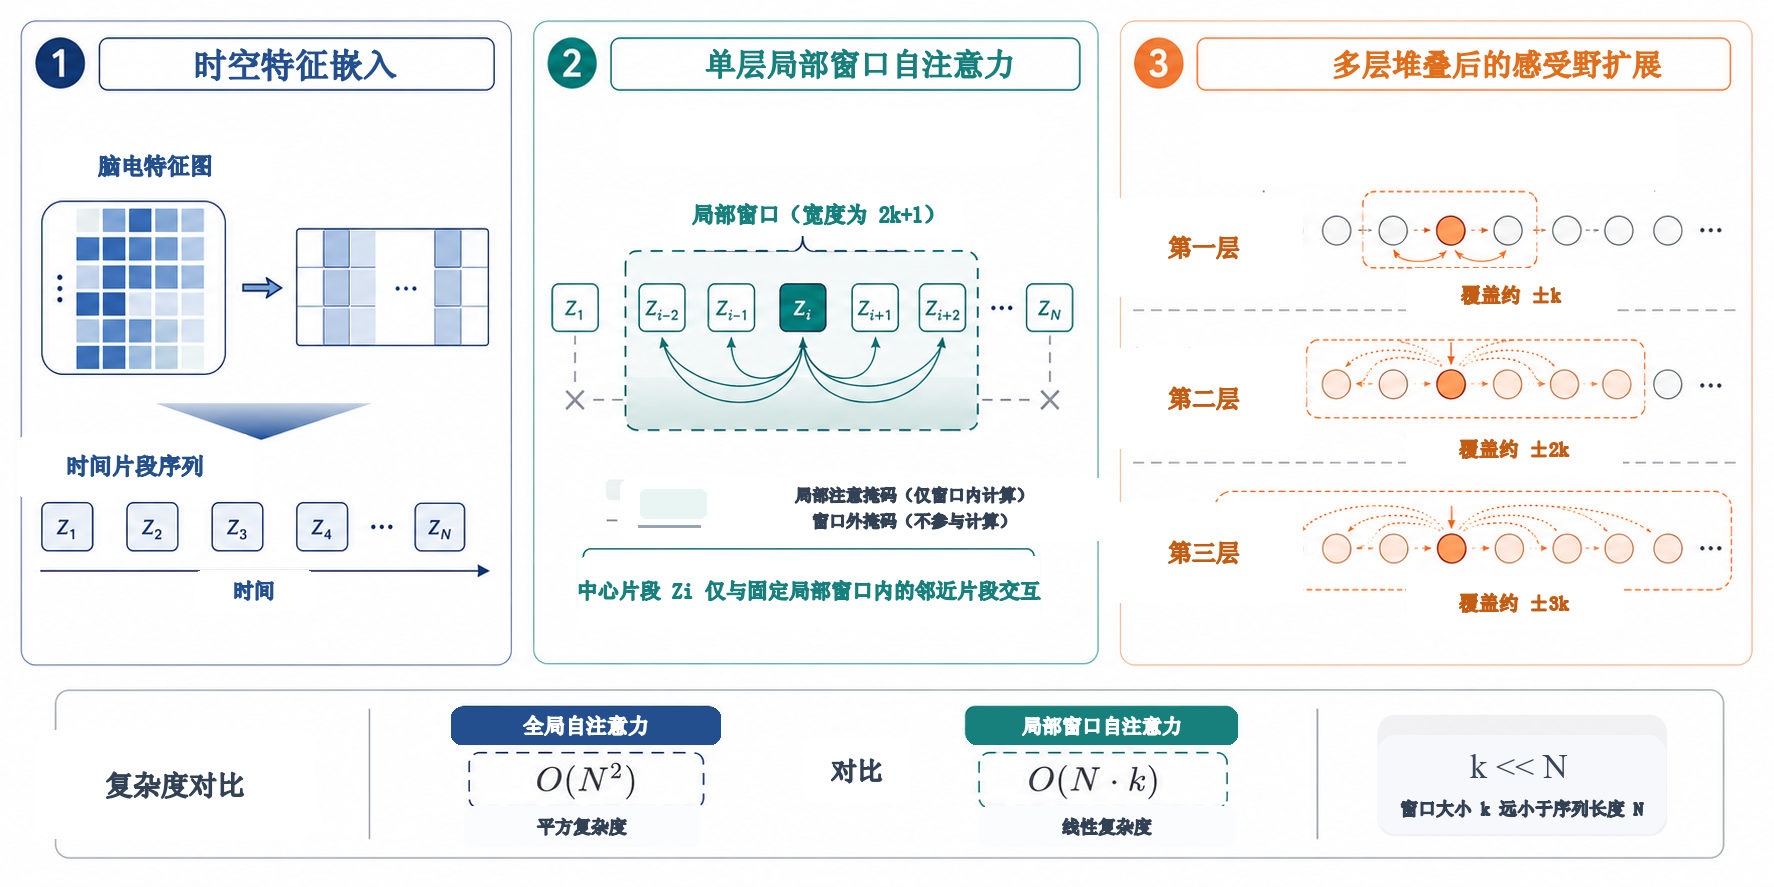
\includegraphics[width=0.97\textwidth]{figures/C4-10_local_window_attention_mechanism.png}
    \caption{局部窗口自注意力与感受野扩展示意}
    \label{fig:chap4_local_window_attention}
\end{figure}

图 \ref{fig:chap4_local_window_attention} 给出了 EdgeMIFormer 中局部窗口自注意力的计算示意。时空特征嵌入后的脑电片段首先被组织为有序时间片段序列；在单层编码器内，中心片段仅与固定局部窗口中的邻近片段发生加权交互，因此注意力计算被限制在局部时间范围内；随着编码器层数增加，局部交互在层间逐步传递，使有效感受野扩展到更长时间上下文。该机制说明，EdgeMIFormer 并非直接对整段序列执行全局两两计算，而是在保持局部结构约束的同时逐步聚合更长程时序信息。

局部窗口自注意力的计算形式可表示为：
\begin{equation}
    A_{local}(Q,K,V)=\text{Softmax}\left(\frac{QK^{T}}{\sqrt{d}}\odot M_{window}\right)V,
    \label{eq:local_attention}
\end{equation}
其中 $Q$、$K$、$V$ 分别为查询、键和值矩阵，$d$ 为嵌入维度，$M_{window}$ 为局部时间窗口掩码，对应图 \ref{fig:chap4_local_window_attention} 中窗口内参与计算、窗口外被屏蔽的约束关系。运动想象脑电的判别线索通常集中在有限时间窗和特定节律范围内，局部窗口自注意力能够为这种局部性提供结构约束，同时降低长序列输入带来的计算负担。

编码器由多层局部窗口自注意力层和前馈网络组成，并通过残差连接保持特征传递的稳定性。对于一层注意力模块，其输出可表示为：
\begin{equation}
    \mathbf{Z}' = \text{LocalAttention}(\mathbf{Z}) + \mathbf{Z}.
    \label{eq:residual}
\end{equation}
该结构在不显著增加模型规模的前提下扩大有效感受野，使底层局部节律表征能够在后续层中进一步组合。分类解码阶段结合全局平均池化、多尺度最大池化和 ELU 激活的全连接层，将时间嵌入映射为运动想象类别概率。由此，模型在标准输入和少导联输入之间共享同一主干，便于比较导联配置和任务定义变化对结果的影响。

训练过程中，模型结合面向脑电信号的增强与优化策略。Segmentation and Reconstruction 将同类试次中的多个 1 s 片段重组以增加时间多样性，SpecAugment 通过时间扰动和随机通道 dropout 模拟电极噪声和佩戴差异。优化器采用 AdamW 与余弦退火策略，并结合标签平滑降低小样本过拟合风险。总体损失由交叉熵损失和最大均值差异（Maximum Mean Discrepancy, MMD）约束组成：
\begin{equation}
    \mathcal{L}=\mathcal{L}_{CE}+0.1\mathcal{L}_{MMD}.
    \label{eq:edgemiformer_training_loss}
\end{equation}
训练增强概率采用课程学习方式由 10\% 逐步增加至 50\%，使模型先学习基础判别模式，再逐步适应更强扰动样本。

\section{实验结果与分析}
\subsection{标准四分类结果与算法有效性分析}
标准四分类实验用于验证 EdgeMIFormer 在完整空间观测条件下的基本解码能力。本章主要实验采用 BCI Competition IV 2a 数据集。该数据集包含 9 名健康受试者的 22 导脑电信号，任务类别包括左手、右手、双脚和舌头四类运动想象，采样率为 250 Hz。数据读取阶段从每个试次中截取 1000 个采样点形成 $1000 \times 22$ 的输入片段，并对异常空值进行置零处理。预处理采用 $4\sim40$ Hz 带通滤波和逐通道标准化，以保留运动想象相关节律并降低跨通道幅值差异。表 \ref{tab:chap4_protocol} 给出了 2a 主实验采用的统一协议。

\begin{table}[htbp]
    \centering
    \caption{BCI Competition IV 2a 主实验的统一协议}
    \label{tab:chap4_protocol}
    \begin{tabular}{cc}
        \hline
        项目 & 设置 \\
        \hline
        数据集 & BCI Competition IV 2a \\
        训练/测试划分 & \texttt{A0xT} / \texttt{A0xE} \\
        建模方式 & 单被试训练，单被试测试 \\
        标准化方式 & 训练集统计量标准化测试集 \\
        随机种子 & 42 \\
        预处理 & $4\sim40$ Hz 带通滤波，逐通道标准化 \\
        输入片段 & 每试次 1000 个采样点 \\
        评价指标 & 分类准确率、模型大小、FLOPs、推理耗时 \\
        \hline
    \end{tabular}
\end{table}

在标准 22 导四分类设置下，表 \ref{tab:chap4_benchmark_comparison} 给出了 EdgeMIFormer 与代表性方法的准确率、模型大小和 FLOPs 对照结果。EdgeMIFormer 的平均最佳准确率为 83.76\%，平均历程准确率为 70.05\%；全局自注意力基线 EEGConformer 的平均最佳准确率为 83.96\%，较 EdgeMIFormer 高 0.20 个百分点，但平均历程准确率低于 EdgeMIFormer 0.07 个百分点；紧凑卷积基线 EEGNet 的平均最佳准确率和平均历程准确率分别为 72.36\% 和 64.56\%。EdgeMIFormer 的模型大小为 1368.35 KB，FLOPs 为 228M，分别低于 EEGConformer 的 1565.62 KB 和 261M。

\begin{table}[htbp]
    \centering
    \caption{标准 22 导四分类结果对比}
    \label{tab:chap4_benchmark_comparison}
    \begin{tabular}{ccccc}
        \hline
        方法 & Avg Best Acc/\% & Avg Aver Acc/\% & 模型大小/KB & FLOPs/M \\
        \hline
        EEGNet & 72.36 & 64.56 & 77.73 & 103 \\
        EEGConformer & 83.96 & 69.98 & 1565.62 & 261 \\
        EdgeMIFormer & 83.76 & 70.05 & 1368.35 & 228 \\
        \hline
    \end{tabular}
\end{table}

上述结果表明，EdgeMIFormer 在标准 22 导四分类任务上达到与 EEGConformer 相近的准确率，同时在模型大小和 FLOPs 上保持更低开销。该实验验证了所提出模型具备有效的运动想象解码能力，也为后续围绕窗口长度、部署压缩和低导联输入展开分析提供了算法基础。

\subsection{窗口长度消融与部署压缩分析}
在标准任务准确率得到验证后，本节进一步分析局部窗口长度和部署压缩对模型规模与推理开销的影响。窗口长度实验关注结构参数对准确率和计算范围的影响，剪枝量化实验关注模型在边缘设备上的存储与推理代价，两组实验共同用于评估 EdgeMIFormer 的端侧适配能力。

局部自注意力窗口大小对准确率表现具有直接影响。窗口大小消融实验比较相同模型结构下不同 $k$ 值的相对变化，与表 \ref{tab:chap4_benchmark_comparison} 中的标准 22 导方法对照共同构成结构有效性证据。在嵌入输出维度为 61 的设置下，窗口大小由 1 增至 9 时，准确率由 79.04\% 提升至 83.77\%，最大准确率为 83.81\%；在嵌入输出维度为 31 的设置下，窗口大小由 1 增至 13 时，准确率由 80.38\% 提升至 83.82\%。图 \ref{fig:window_size_ablation} 中的误差条表示三次独立实验的标准差。结果表明，窗口较小时扩大局部窗口能够引入更充分的时间上下文并提升准确率；窗口增加到一定范围后，继续扩大窗口带来的准确率收益趋于饱和。该结果反映保持合适的局部窗口长度能够在保持准确率的同时减少注意力机制的计算范围。

\begin{figure}[H]
    \centering
    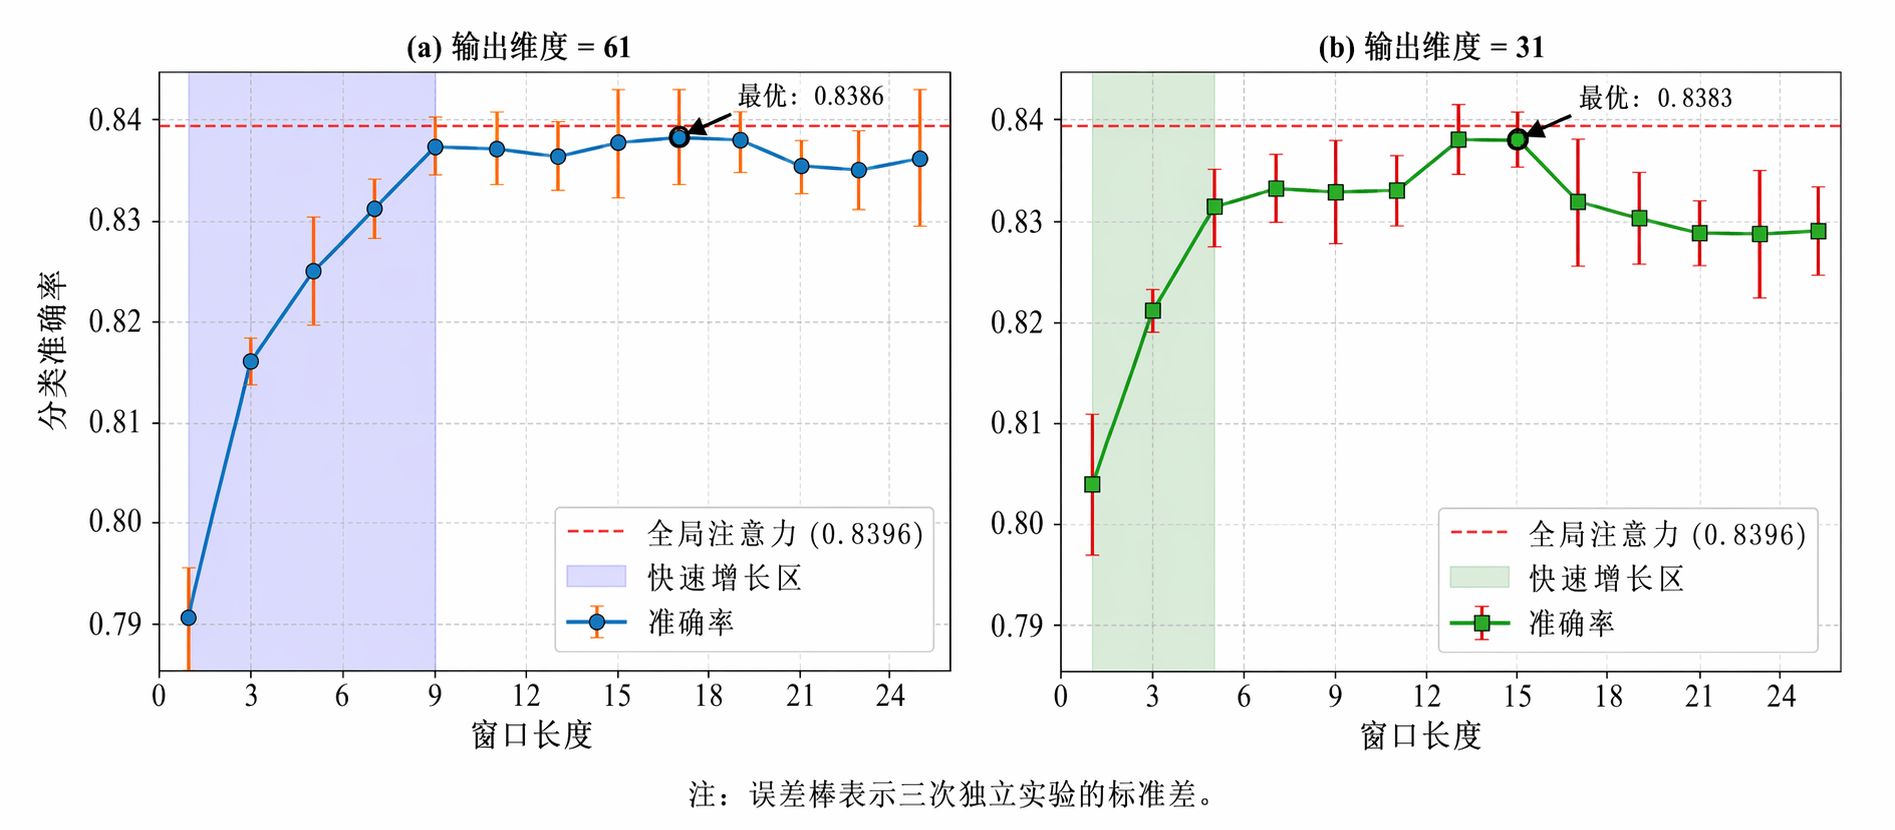
\includegraphics[width=\textwidth]{figures/C4-11_window_size_ablation.png}
    \caption{局部自注意力窗口长度对标准 22 导四分类准确率的影响}
    \label{fig:window_size_ablation}
\end{figure}

模型规模控制通过模型大小、FLOPs 和推理耗时衡量。部署流程采用 PyTorch 模型导出 ONNX，再通过 RKNN Toolkit 转换为 RKNN 模型，并在转换过程中结合结构化剪枝与量化。具体而言，模型采用基于 L1 范数排序的 30\% 全局结构化通道剪枝，并进一步比较非对称量化与 KL 散度对称量化两种方案。

表 \ref{tab:chap4_deployment_result} 给出了不同部署版本的准确率、模型大小和推理耗时。该表用于比较剪枝、量化和 RK NPU 部署对模型推理环节的影响，与标准 22 导对照和少导联重跑实验采用不同测试协议。原始模型在 CPU 上的推理耗时为 683360 $\mu$s，在 RK NPU 上降至 44700 $\mu$s，准确率保持为 83.76\%。在 30\% 结构化剪枝基础上，非对称量化将模型大小压缩至 810.56 KB，推理耗时降至 31729 $\mu$s，但准确率下降至 83.19\%；KL 散度对称量化后的模型大小进一步降至 655.36 KB，仅为原始模型的 47.9\%，推理耗时为 31314 $\mu$s，约为 31 ms，同时准确率仍保持在 83.42\%。

\begin{table}[htbp]
    \centering
    \caption{剪枝量化与 RK NPU 部署结果}
    \label{tab:chap4_deployment_result}
    \begin{tabular}{cccc}
        \hline
        模型版本 & 准确率/\% & 模型大小/KB & 推理耗时/$\mu$s \\
        \hline
        Original (CPU) & 83.76 & 1368.35 & 683360 \\
        Original (NPU) & 83.76 & 1368.35 & 44700 \\
        Asymmetric Quantization & 83.19 & 810.56 & 31729 \\
        KL Symmetric Quantization & 83.42 & 655.36 & 31314 \\
        \hline
    \end{tabular}
\end{table}

上述结果表明，EdgeMIFormer 在采用结构化剪枝与 KL 散度对称量化后，相较原始模型准确率仅下降 0.34 个百分点，模型大小减少约 52.1\%。局部窗口长度控制了自注意力计算范围，结构化剪枝和 KL 对称量化进一步降低了模型存储和推理代价。两类结果共同说明，EdgeMIFormer 在保持标准任务准确率的同时具备低开销推理与模型侧部署基础，但这一结论仍限定在离线部署测试与模型转换证据范围内。

\subsection{低导联性能边界与任务收束分析}
本节围绕导联受限条件下的输入形态和任务类别粒度展开实验分析。该实验链条关注一个核心问题：当输入导联被压缩到中央区少量电极时，原始四分类任务是否仍能保持有效判别，以及 C3/C4 双导条件下更合适的任务类别粒度应如何确定。

本文在保持数据集、训练测试划分、标准化方式和评价指标一致的前提下，对输入导联数进行逐级压缩。表 \ref{tab:channel_degradation} 给出了 22 导、8 导、3 导和 2 导四分类任务的平均结果。随着输入导联从标准 22 导逐步减少到中央区少量导联，平均最佳准确率由 83.76\% 依次下降至 72.08\%、62.88\% 和 49.73\%，累计降幅达到 34.03 个百分点；平均历程准确率也由 70.05\% 降至 44.41\%。该结果呈现了导联数量减少时四分类任务表现的变化趋势，说明双导输入下直接保留四分类会面临明显信息约束。

\begin{table}[htbp]
    \centering
    \caption{导联逐级压缩条件下四分类性能变化}
    \label{tab:channel_degradation}
    \begin{tabular}{cccc}
        \hline
        导联配置 & 导联数 & Avg Best Acc/\% & Avg Aver Acc/\% \\
        \hline
        全通道 & 22 & 83.76 & 70.05 \\
        中央区 8 导 & 8 & 72.08 & 61.28 \\
        C3/Cz/C4 三导 & 3 & 62.88 & 51.70 \\
        C3/C4 双导 & 2 & 49.73 & 44.41 \\
        \hline
    \end{tabular}
\end{table}

从变化幅度看，22 导到 8 导阶段下降约 11.68 个百分点，8 导到 3 导阶段下降约 9.20 个百分点，3 导到 2 导阶段进一步下降约 13.15 个百分点。前两个阶段的下降相对平缓，说明中央区周围仍保留一定数量导联时，模型仍能利用感觉运动皮层及相邻区域的空间判别线索；当输入进一步压缩为 C3/C4 双导时，空间观测范围显著缩小，四分类任务中的部分类别边界随之变弱。导联压缩实验由此给出了低导联四分类的性能边界。

在确认双导四分类受限后，本文保持 C3/C4 双导输入不变，仅将任务从四分类收束为左右手二分类。表 \ref{tab:c3c4_task_redefine} 显示，C3/C4 双导二分类的平均最佳准确率达到 70.76\%，平均历程准确率为 64.88\%，相较于双导四分类分别提升 21.03 和 20.47 个百分点。由于输入导联没有增加，该改善来自任务目标与 C3/C4 可稳定观测侧化运动想象信息之间的重新匹配。

\begin{table}[htbp]
    \centering
    \caption{C3/C4 双导条件下四分类与左右手二分类性能对比}
    \label{tab:c3c4_task_redefine}
    \begin{tabular}{ccc}
        \hline
        任务设置 & Avg Best Acc/\% & Avg Aver Acc/\% \\
        \hline
        C3/C4 双导四分类 & 49.73 & 44.41 \\
        C3/C4 双导二分类 & 70.76 & 64.88 \\
        \hline
    \end{tabular}
\end{table}

C3/C4 主要覆盖左右感觉运动皮层，对左右手运动想象诱发的侧化节律变化更敏感；双脚与舌头类别涉及中线附近或更广范围的空间分布。在仅保留 C3/C4 双导时，左右手二分类更符合导联位置的生理可观测性。表 \ref{tab:c3c4_task_redefine} 的结果表明，任务类别粒度调整能够在不增加输入导联的条件下显著恢复双导解码性能。

类别级错误结构能够更直接地解释任务收束的必要性。图 \ref{fig:confusion_key_conditions} 汇总了 22 导四分类、C3/C4 双导四分类和 C3/C4 双导左右手二分类三种关键设置的类别级识别结果。结果表明，在 22 导四分类条件下，四类召回率分别为 72.38\%、74.54\%、75.62\% 和 71.14\%，整体较为均衡；在 C3/C4 双导四分类条件下，左手、右手、双脚和舌头四类召回率分别降至 56.02\%、47.38\%、38.73\% 和 56.79\%。双脚类和右手类退化幅度更大，说明双导空间压缩会优先影响更依赖中线区域或广域空间分布的类别判别。

\begin{figure}[H]
    \centering
    
\includegraphics[width=0.88\textwidth]{C4-12_confusion_matrix_key_conditions.png}
    \caption{关键条件下的聚合混淆矩阵}
    \label{fig:confusion_key_conditions}
\end{figure}

当任务目标收束为左右手二分类后，左右手类别召回率恢复到 72.99\% 和 68.52\%。结合表 \ref{tab:c3c4_task_redefine} 和图 \ref{fig:confusion_key_conditions}，双导输入下的性能改善主要来自任务目标与 C3/C4 可观测侧化信息之间的重新匹配。

为补充验证低导联左右手二分类任务的外部可行性，本文进一步引入 BCI Competition IV 2b 数据集结果。BCI IV 2b 是左右手二分类运动想象数据集，当前实验采用 C3/Cz/C4 三导输入。该设置与 BCI IV 2a 中的 C3/C4 双导二分类在导联数和数据协议上存在差异，因此在本文中承担跨数据集补充验证作用。表 \ref{tab:bciiv2b_external_result} 显示，EdgeMIFormer 在 BCI IV 2b 的 9 名被试三导二分类设置下，单次实验平均最佳准确率为 82.85\%，平均历程准确率为 78.16\%。多随机种子汇总结果中，平均最佳准确率为 82.84\%$\pm$0.24\%，平均历程准确率为 77.87\%$\pm$0.27\%，表明该低导联二分类结果对随机初始化具有较小波动。

\begin{table}[htbp]
    \centering
    \small
    \caption{BCI IV 2a 与 BCI IV 2b 低导联左右手二分类结果对照}
    \label{tab:bciiv2b_external_result}
    \begin{tabular}{ccccc}
        \hline
        数据集 & 导联配置 & 任务设置 & Avg Best Acc/\% & Avg Aver Acc/\% \\
        \hline
        BCI IV 2a & C3/C4 & 左右手二分类 & 70.76 & 64.88 \\
        BCI IV 2b & C3/Cz/C4 & 左右手二分类 & 82.85 & 78.16 \\
        \hline
    \end{tabular}
\end{table}

综合导联压缩、C3/C4 二分类和 BCI IV 2b 三导二分类结果，低导联实验链条表明，C3/C4 双导难以直接支撑稳定四分类，而左右手二分类能够更好地匹配中央区双导输入的可观测信息。由此，C3/C4 双导左右手二分类可作为后续在线验证的优先任务形式。

\section{本章小结}

本章从算法侧给出了受限采集与边缘算力条件下的运动想象脑电解码模型设计与验证结果。结合运动想象脑电在中央感觉运动区的节律响应特征，本文明确了标准 22 导参考输入、C3/C4 双导目标输入和中间导联数过渡分析之间的关系，并围绕卷积前端、局部窗口自注意力、分类聚合头和训练增强策略构建了 EdgeMIFormer。该模型通过局部窗口自注意力控制注意力机制的计算范围，并保持对不同导联数量输入的基本兼容。

在标准 22 导四分类实验中，EdgeMIFormer 取得 83.76\% 的平均最佳准确率和 70.05\% 的平均历程准确率，与全局自注意力基线 EEGConformer 的平均最佳准确率差距为 0.20 个百分点，同时模型大小和 FLOPs 均低于 EEGConformer。局部窗口长度消融结果表明，在窗口较小的阶段扩大窗口能够提升准确率，窗口继续增大后收益趋于饱和。部署测试表明，在结构化剪枝与 KL 散度对称量化后，模型仍保持 83.42\% 的准确率，模型大小降至 655.36 KB，RK NPU 推理耗时约为 31 ms，说明模型推理环节具备端侧部署基础。

在导联受限实验中，统一协议下的 22 导、8 导、3 导和 2 导四分类结果呈下降趋势，说明导联数量减少会改变四分类任务的可判别信息条件。保持 C3/C4 双导输入不变并将任务收束为左右手二分类后，平均最佳准确率提升至 70.76\%，平均历程准确率提升至 64.88\%。混淆矩阵进一步表明，双脚和舌头等类别更容易受到双导空间压缩影响；BCI IV 2b 三导二分类结果则提供了低导联左右手任务的跨数据集补充证据。总体而言，本章从算法侧给出了标准输入性能、模型侧部署能力和双导目标任务选择的证据，并将 C3/C4 双导左右手二分类确定为后续在线验证的优先任务形式。
